\ifx\isEmbedded\undefined

\documentclass[12pt]{report}
	
% FONT RELATED
%\usepackage{times} %Move to times font
\usepackage[labelfont=bf,textfont=it]{caption}
\usepackage[utf8]{inputenc}

% LINKS, PAGE OF CONTENT, REF AND CROSS-REF, HEADERS/FOOTERS
\usepackage[hidelinks]{hyperref}
\usepackage{fancyhdr}
\usepackage{acronym}

% FIGURES, GRAPHICS, TABLES
\usepackage{graphicx}
\usepackage{parskip}
%\usepackage{subfigure}
\usepackage{subfig}
\usepackage{wrapfig}
\usepackage{subfloat}

% COLOURS, TEXT AND FORMATTING
\usepackage{array}
\usepackage{color}
\usepackage{setspace}
\usepackage{longtable}
\usepackage{multirow}

% ADVANCED MATHS, PSEUDO-CODE
\usepackage{amsmath}
\usepackage{alltt}
\usepackage{amsfonts}

% BIBLIOGRAPHY
\usepackage[authoryear]{natbib}
\bibpunct{(}{)}{;}{a}{,}{,}

% USE IN DISSER:

\setlength\oddsidemargin{0.85cm}
\setlength\evensidemargin{0.85cm}

\setlength\textheight{21.0cm}
\setlength\textwidth{15.0cm}

% indent at each new paragrapg
\setlength\parindent{0.5cm}

\setlength\topmargin{-0.2in}
\renewcommand{\baselinestretch}{1.3}

%REPORT

%\setlength\oddsidemargin{1cm}
%\setlength\evensidemargin{0.3in}
%%\setlength\headsep{2.5in}
%
%\setlength\textheight{9.0in}
%\setlength\textwidth{5.5in}
%
%% indent at each new paragrapg
%\setlength\parindent{0.5cm}
%
%%\setlength{\parskip}{10.5ex}
%
%\setlength\topmargin{-0.2in}

%\newcommand{\HRule}{\rule{\linewidth}{0.5mm}}
\newcommand{\HRule}{\rule{\linewidth}{0.0mm}}

% Color definitions (RGB model)
\definecolor{ms-comment}{rgb}{0.1, 0.4, 0.1}
\definecolor{ms-question}{rgb}{0.4, 0.0, 0.0}
\definecolor{ms-new}{rgb}{0.2, 0.4, 0.8}


\graphicspath{{../img/}}
\begin{document}
\fi

\chapter{Technical Background}
\label{chap:technical_background}

The background needed for doing research on engineering or any technical discipline is extremely important, and frequently is what marks the difference between a solid, consistent and robust study from a weak one. Many mathematical and physical concepts (specially physical) are critical to understand analytically the ideas, reasoning and logical models presented in this survey.

This chapter intends to describe formally the main ground concepts where this thesis is settled on. Although this may only be a brief glimpse of all the ideas applied directly or indirectly, and a much finer conceptual background might be developed, this should be enough for following the approach.

The bibliography resource consulted to write this section was the chapter A Maths and Physics Primer, in the book Programming Game AI by Example \citep{buckland}.

\section{Physics}

In any research that involves modelling the real world, physical rules will acquire a fundamental role, particularly the ones concerned with motion. Next, the key concepts to understand the virtual force model will be presented.

\begin{itemize}

\item{{\bf Time.} This is a concept that everybody has in mind. Physically speaking, time is a dimension in which events can be ordered from the past through the present into the future. It is a continuous scalar quantity with no direction measured in seconds. Time in computer simulations and computer games might be measured in seconds, like in the real world, or in \emph{virtual seconds} or \emph{ticks}. This will be discussed more in depth in Chapter \ref{chap:application_design_implementation}: Application Design and Implementation.}

\item{{\bf Mass.} It is a scalar quantity measured in grams, and it is the measure of an amount of something. This property is directly linked to how fast bodies change of state. For example, if we imagine two people with the same properties except mass, the one with higher mass will require more time to change from standing to running.}

\item{{\bf Strength.} It is the scalar quantity which defines the physical power a person or animal has. Notice that this property is inherent to an individual and does not have direction, if it had, we would be talking about \emph{force}, concept that will be introduced later. And again, this is related with how fast bodies change of state. The bigger strength, the faster change.}

\item{{\bf Position.} These are the location coordinates of a specific point related to an origin. This is not as simple as it might seem, because bodies have a volume, so which the exact position is, is a controversial discussion. Normally it is used the centre of mass, but other points can be used depending on the approach. In order to calculate the movement, we need to know the rate of change of the position, both the magnitude and the direction.}

\item{{\bf Velocity.} This is the vector which defines the rate of change of distance over time. Its standard unit of measurement is $m/s$. Mathematically it can be expressed as follows:}

\begin{equation}
  v=\frac{\Delta x}{\Delta t}
\end{equation}

\item{{\bf Acceleration.} It is a vector which defines the rate of change of velocity over time. Acceleration is written as $m/s^2$, and expressed by:}

\begin{equation}
  a=\frac{\Delta v}{\Delta t}
\end{equation}

\item{{\bf Force.} This is the main element of the physical model followed by this thesis. 
 According to Isaac Newton: ``An impressed force is an action exerted upon a body in order to change its state, either of rest, or of uniform motion in a right line''.
 Therefore, a force is a quality that can alter an object's speed or line of motion. It is measured in Newtons and represented as a vector, with both magnitude and direction}

\end{itemize}

We know that to change the position of an object (to move it), it is needed to make its velocity greater than 0, and in order to achieve that, there has to exist an acceleration. Basically, what the object is experimenting is a change of state due to an acceleration produced by forces.

Newton's second law states the relatioship between an object's mass m, its acceleration a, and the applied force F by the equation:

\begin{equation}
  F=ma
\end{equation}

%\newpage
Therefore, this gives us the key to perform a physically based simulation. According to all mentioned before, the motion an object experiments in a physically based virtual world can be calculated after synthesizing all the forces applied over it:

\begin{enumerate}
%\centering
\item $a = \frac{F_{total}}{m}$
\item $v_{t+1} = v_{t}+a$
\item $p_{t+1} = p_{t}+v_{t+1}$
\end{enumerate}

\section{Reynold's Flocking Algorithm}

Craig W. Reynolds proposed in 1987 a model to simulate natural group behaviours such as herds, flocks or schools \citep{reynolds}. This is a very powerful mechanism to use in crowds, besides sharing the principles this thesis is based on. The method works by applying three simple rules to each individual of the flock, which Reynolds called \emph{boids}, that make them move as a unit.

\begin{figure}[!h]
  \centering
  \begin{tabular}{c c c}
  	\subfloat[Cohesion Rule]{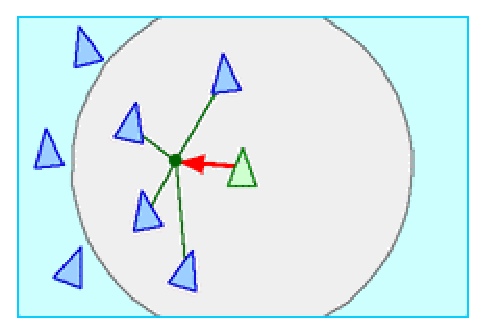
\includegraphics[scale=0.6]{cohesion.eps}} &
 	\subfloat[Separation Rule]{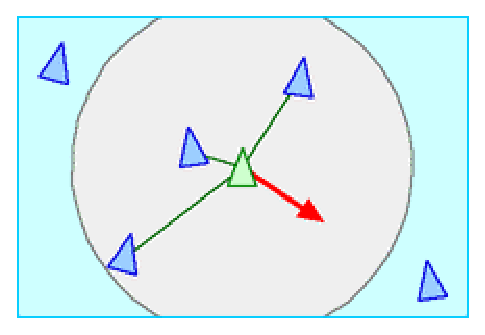
\includegraphics[scale=0.6]{separation.eps}} &
  	\subfloat[Alignment Rule]{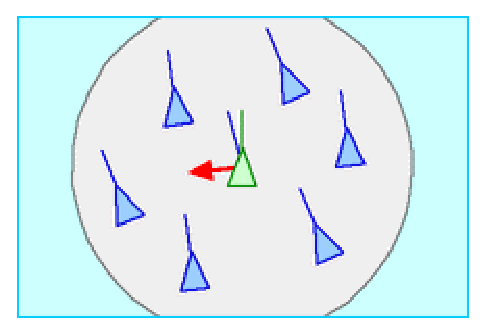
\includegraphics[scale=0.6]{alignment.eps}} \\
 \end{tabular}
  \caption{Reynolds' Model Rules}
  \label{fig:crowds}
\end{figure}

Each boid knows a set of neighbours in the flock which influence its movement. Only the ones that are within a certain distance are considered neighbours, and the rest are ignored; thus, boids has local conscience of the flock. According to the virtual force model, those simple rules produce these three steering forces:

\begin{itemize}

\item{{\bf Cohesion.} This force makes the boid move towards the centre of mass of the neighbourhood so that they remain close to each other.\\

Let $p$ be the position and $v$ the velocity of the current boid, $p_i$ the position of the neighbour i and $n$ the number of neighbours:

\begin{equation}
  centreOfMass=\frac{\sum_{i=1}^np_i}{n}
\end{equation}

\begin{equation}
  cohesionForce=normalize(centreOfMass-p)maxSpeed-v
\end{equation}
}

\item{{\bf Separation.} This force makes the boid move away from its neighbours, to avoid remaining too close.\\

Let $p$ be the position of the current boid, $p_i$ the position of the neighbour i, $d_i$ the distance to the neighbour i and $n$ the number of neighbours:

\begin{equation}
  separationForce=\sum_{i=1}^n\frac{normalize(p-p_i)}{d_i}
\end{equation}
}

\item{{\bf Alignment.} This attemps to keep the boid aligned with their neighbours.\\

Let $p$ be the position and $v$ the velocity of the current boid, $p_i$ the position and $v_i$ the velocity of the neighbour i and $n$ the number of neighbours:

\begin{equation}
  averageHeading=\frac{\sum_{i=1}^nnormalize(v_i)}{n}
\end{equation}

\begin{equation}
  alignmentForce=averageHeading-normalize(v)
\end{equation}
}

\end{itemize}

\section{Finite State Machine (FSM)}

Finite State Machines, or FSM, have been the main instrument of choice to imbue an agent the illusion on intelligence. Some of the reasons are these:

\begin{itemize}
\item{Quick and simple to code}
\item{Easy to debug}
\item{Little computational overhead}
\item{They are intuitive}
\item{They are flexible}
\end{itemize}

Historically, a FSM is a rigidly formalized device used by mathematicians to solve problems, whose precursor might be considered the Turing Machine. The idea is to decompose an object's behaviour into easily manageable ``chunks'' or states. For instance, a light switch is a very simple FSM where \emph{off} and \emph{on} are the states. Transitions are made by the input of the fingers. By clicking the switch up it triggers the transition from off to on, and by clicking the switch down it triggers the transition from on to off. There is no action associated with the off state, but when it is on, the electricity is allowed to flow and light up the room.

\begin{figure}[!htb]
  \centering
  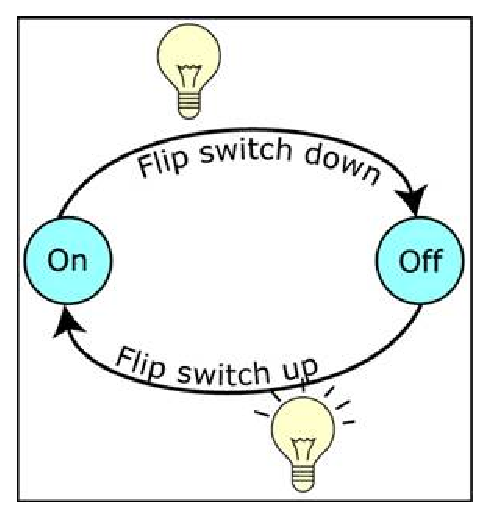
\includegraphics[scale=0.6]{fsm.eps}
  \caption{Light Finite State Machine}
  \label{fig:light}
\end{figure}

As mentioned above, one of the main advantages of FSM is that they are very intuitive. It is human nature to think about things as being in one state or another. Humans do not really work like FSM but sometimes it is useful to think our behaviour in this way. It is fairly easy to break down an agent's behaviour into a number of states with associated actions and to create rules to transit among them.

One feature that notably enhance the power of FSM and allow intercommunication among agents is the message passing support. Intelligent agents can send and receive information to each other, and act upon it. This is a model which reflects quite accurately how real interactions work. This messages are sent in the form of packets of data to other agents, which might influence their behaviour triggering a transition to a different state. If an archer sends an ``arrow'' message to an enemy, this might respond changing his state from alive to dead.

\ifx\isEmbedded\undefined
% References
\addcontentsline{toc}{chapter}{References}
\bibliographystyle{../ref/harvard}
\bibliography{../ref/master}
\pagebreak
\end{document}
\fi